\chapter{Discussion}
Please tell more about conclusion and how to the next work of this study.

\section{Ahmad Syafrizal Huda/1164062}
\subsection{Teori}
\begin{enumerate}
\item Jelaskan kenapa file suara harus di lakukan MFCC.
\subitem File suara harus dilakukan MFCC(Mel Frequency Cepstral Coeficients) karena MFCC dapat mengubah file suara/frekuensi suara ke dalam bentuk data vektor yang nantinya akan diolah menjadi outputan dimana telah dilakukan ekstraksi oleh MFCC kemudian direalisasikan sebagai data matrix. Contoh ilustrasi dapat dilihat pada gambar \ref{c6_1}.
\begin{figure}[!htbp]
	\centerline{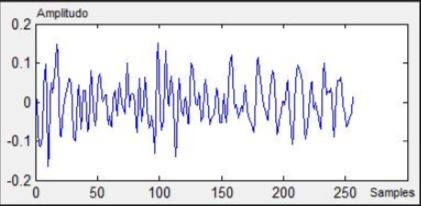
\includegraphics[width=1\textwidth]{figures/huda/chapter6/1.JPG}}
	\caption{Suara ke MFCC}
	\label{c6_1}
\end{figure} 
\item Jelaskan konsep dasar neural network.
\subitem Neural Network merupakan sistem komputasi yang efisien dimana tema utamanya dipinjam dari analogi jaringan saraf biologis. Neural Network biasa disebut dengan jaringan saraf tiruan dimana Neural Network sebenarnya mengadopsi dari kemampuan otak manusia yang mampu memberikan stimulasi/rangsangan, melakukan proses, dan memberikan output. Contoh ilustrasi dapat dilihat pada gambar \ref{c6_2}.
\begin{figure}[!htbp]
	\centerline{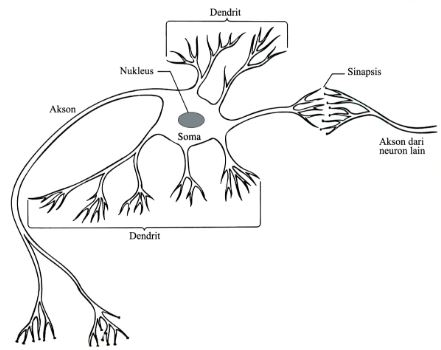
\includegraphics[width=1\textwidth]{figures/huda/chapter6/2.JPG}}
	\caption{Neural Network}
	\label{c6_2}
\end{figure} 
\item Jelaskan konsep pembobotan dalam neural network.
\subitem Sebuah Neural Network dikonfigurasi untuk aplikasi tertentu, seperti pengenalan pola atau klasifikasi data, contohnya pada Neural Network melakukan penyesuaian koneksi sinaptik antar neuron dilakukan dengan menyesuaikan nilai bobot yang ada pada tiap konektivitas baik dari input, neuron maupun output disinkronkan dengan penyesuaian koneksi sinaptik antar neuron itu sendiri. Contoh ilustrasi dapat dilihat pada gambar \ref{c6_3}.
\begin{figure}[!htbp]
	\centerline{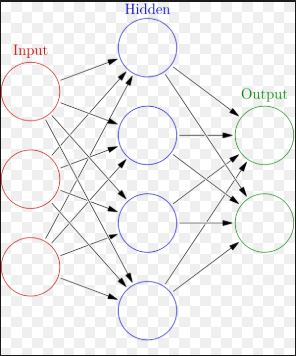
\includegraphics[width=1\textwidth]{figures/huda/chapter6/3.JPG}}
	\caption{Pembobotan Neural Network}
	\label{c6_3}
\end{figure} 
\item Jelaskan konsep fungsi aktifasi dalam neural network.
\subitem Fungsi aktivasi dalam neural network yaitu setiap neuron mempunyai tingkat aktivasi yang merupakan fungsi dari input yang masuk padanya. Aktivasi yang dikirim suatu neuron ke neuron lain berupa sinyal dan hanya dapat mengirim sekali dalam satu waktu, meskipun sinyal tersebut disebarkan pada beberapa neuron yang lain. Contoh ilustrasi dapat dilihat pada gambar \ref{c6_4}.
\begin{figure}[!htbp]
	\centerline{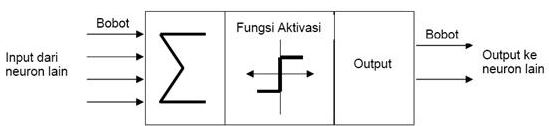
\includegraphics[width=1\textwidth]{figures/huda/chapter6/4.JPG}}
	\caption{Aktivasi Neural Network}
	\label{c6_4}
\end{figure} 
\item Jelaskan cara membaca hasil plot dari MFCC.
\subitem Cara membaca hasil plot dari MFCC yaitu Nanti akan ada outputan berbentuk grafik setelah melakukan plot dari MFCC. Kemudian terdapat frekuensi/Hz pada suara frekuensi biasanya vertikal atau biasa disimbolkan dengan sumbu y, Lalu terdapat waktu yang mana waktu diartikan dalam simbol sumbu x. Sedangkan pada bagian dalam atau bisa disimbolkan dengan sumbu z merupakan power atau kekuatan dari lagu atau suara atau desibel yang dihasilkan. Untuk warna biru itu merupakan suara rendah, yang merah merupakan tinggi apabila daya frekuensi nya misalkan suara siul berarti dominan warna merah karena siul biasanya pada nada yang tinggi sedangkan jika bass dominan biru karena bass merupakan nada rendah. Contoh ilustrasi dapat dilihat pada gambar \ref{c6_5}.
\begin{figure}[!htbp]
	\centerline{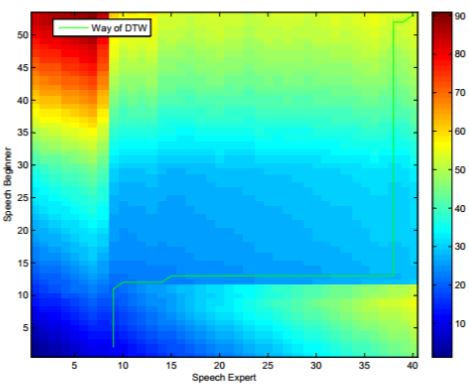
\includegraphics[width=1\textwidth]{figures/huda/chapter6/5.JPG}}
	\caption{Membaca Hasil Plot dari MFCC}
	\label{c6_5}
\end{figure} 
\item Jelaskan apa itu one-hot encoding.
\par One-hot encoding adalah representasi dari variabel kategori sebagai vektor biner. Yaitu nilai kategorika harusl dipetakan ke nilai integer. Kemudian, setiap nilai integer direpresentasikan sebagai vektor biner yang semuanya bernilai nol kecuali indeks integer, yang ditandai dengan 1. Contoh ilustrasi dapat dilihat pada gambar \ref{c6_6}.
\begin{figure}[!htbp]
	\centerline{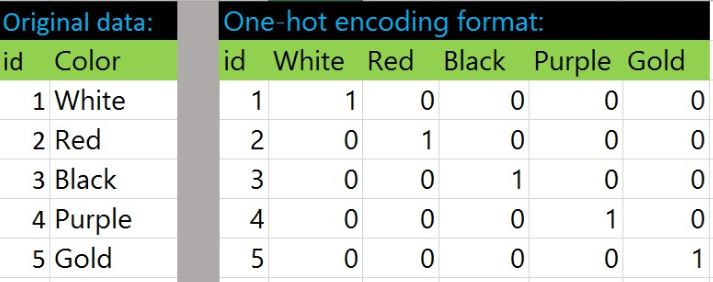
\includegraphics[width=1\textwidth]{figures/huda/chapter6/6.JPG}}
	\caption{One-Hot Encoding}
	\label{c6_6}
\end{figure} 
\item Jelaskan apa fungsi dari np.unique dan to\_categorical dalam kode program.
\begin{itemize}
\item np.unique untuk mengekstaksi elemen-elemen unik tertentu dalam array.
\item to\_categorical untuk mengubah vektor kelas yang berupa integer menjadi matriks kelas biner.
\end{itemize}
\begin{figure}[!htbp]
	\centerline{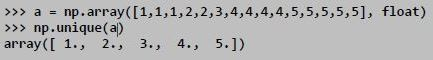
\includegraphics[width=1\textwidth]{figures/huda/chapter6/7.JPG}}
	\caption{np.unique}
\end{figure} 
\begin{figure}[!htbp]
	\centerline{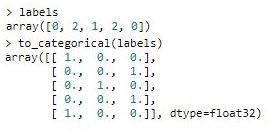
\includegraphics[width=1\textwidth]{figures/huda/chapter6/7_1.JPG}}
	\caption{to\_categorical}
\end{figure} 
\item Jelaskan apa fungsi dari Sequential dalam kode program.
\subitem Fungsi dari Sequential dalam kode program yaitu meruapakan sebuah jenis model yang digunakan dalam perhitungan ataupun code program yang direalisasikan. Neural Networks Sequential membangun fitur tingkat tinggi melalui lapisan yang berurutan. Sequential juga merupakan proses dimana membandingkan setiap elemen larik satu per satu secara beruntun, mulai dari elemen pertama, sampai dengan elemen terakhir atau elemen yang dicari sudah ditemukan.  Contoh ilustrasi dapat dilihat pada gambar \ref{c6_8}.
\begin{figure}[!htbp]
	\centerline{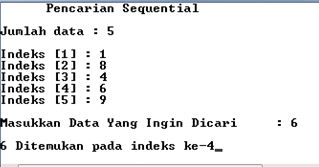
\includegraphics[width=1\textwidth]{figures/huda/chapter6/8.JPG}}
	\caption{One-Hot Encoding}
	\label{c6_8}
\end{figure} 
\end{enumerate}

\subsection{Praktek Program}
\begin{enumerate}
\item Jelaskan isi dari data GTZAN Genre Collection dan data dari freesound. Buat kode program untuk meload data tersebut untuk digunakan pada MFCC.
\item Jelaskan perbaris kode program dengan kata-kata dan dilengkapi ilustrasi gambar fungsi dari display mfcc() .
\item Jelaskan perbaris kode program dengan kata-kata dan dilengkapi ilustrasi gambar fungsi dari extract features song(). Jelaskan juga mengapa yang diambil 25.000 baris pertama?
\item Jelaskan perbaris kode program dengan kata-kata dan dilengkapi ilustrasi gambar fungsi dari generate features and labels().
\item Jelaskan dengan kata dan praktek kenapa penggunaan fungsi generate features and labels() sangat lama ketika meload dataset genre.
\item Jelaskan kenapa harus dilakukan pemisahan data training dan data set sebesar 80 persen?
\item Praktekkan dan jelaskan masing-masing parameter dari fungsi Sequential().
\item Praktekkan dan jelaskan masing-masing parameter dari fungsi compile() dan tunjukkan keluarannya dengan fungsi summary.
\item Praktekkan dan jelaskan masing-masing parameter dari fungsi fit().
\item Praktekkan dan jelaskan masing-masing parameter dari fungsi evaluate().
\item Praktekkan dan jelaskan masing-masing parameter dari fungsi predict(). 
\end{enumerate}

\subsection{Penanganan Eror}
\begin{enumerate}
\item ScreenShoot Error
\item Tuliskan kode eror dan jenis errornya.
\item Solusi pemecahan masalah error tersebut.
\end{enumerate}
